\documentclass[11pt,a4paper]{article}
\usepackage[utf8]{inputenc}
\usepackage[french]{babel}
\usepackage[T1]{fontenc}

\usepackage{amsmath}
\usepackage{amsfonts}
\usepackage{amssymb}

\newcommand{\NomAuteur}{Fabrice BOISSIER}
\newcommand{\TitreMatiere}{Architecture des Ordinateurs 1}
\newcommand{\NomUniv}{EPITA - Bachelor Cyber Sécurité}
\newcommand{\NiveauUniv}{CYBER1}
\newcommand{\NumGroupe}{CYBER1}
\newcommand{\AnneeUniv}{2024-2025}
\newcommand{\DateExam}{27 janvier 2025}
\newcommand{\TypeExam}{Partiel (Sujet B)}
\newcommand{\TitreExam}{\TitreMatiere}
\newcommand{\DureeExam}{1h30}
\newcommand{\MyWaterMark}{\AnneeUniv} % Watermark de protection

% Ajout de mes classes & definitions
\usepackage{MetalExam} % Appelle un .sty

% "Tableau" et pas "Table"
\addto\captionsfrench{\def\tablename{Tableau}}

%%%%%%%%%%%%%%%%%%%%%%%
%Header
%%%%%%%%%%%%%%%%%%%%%%%
\lhead{\TypeExam}							%Gauche Haut
\chead{\NomUniv}							%Centre Haut
\rhead{\NumGroupe}							%Droite Haut
\lfoot{\DateExam}							%Gauche Bas
\cfoot{\thepage{} / \pageref*{LastPage}}	%Centre Bas
\rfoot{\texttt{\TitreMatiere}}				%Droite Bas

%%%%%

\usepackage{tabularx}

\newlength{\LabelWidth}%
%\setlength{\LabelWidth}{1.3in}%
\setlength{\LabelWidth}{1cm}%
%\settowidth{\LabelWidth}{Employee E-mail:}%  Specify the widest text here.

% Optional first parameter here specifies the alignment of
% the text within the \makebox.  Default is [l] for left
% alignment. Other options are [r] and [c] for right and center
\newcommand*{\AdjustSize}[2][l]{\makebox[\LabelWidth][#1]{#2}}%


\definecolor{mGreen}{rgb}{0,0.6,0}
\definecolor{mGray}{rgb}{0.5,0.5,0.5}
\definecolor{mPurple}{rgb}{0.58,0,0.82}
\definecolor{backgroundColour}{rgb}{0.95,0.95,0.92}

\lstdefinestyle{CStyle}{
    backgroundcolor=\color{backgroundColour},
    commentstyle=\color{mGreen},
    keywordstyle=\color{magenta},
    numberstyle=\tiny\color{mGray},
    stringstyle=\color{mPurple},
    basicstyle=\footnotesize,
    breakatwhitespace=false,
    breaklines=true,
    captionpos=b,
    keepspaces=true,
    numbers=left,
    numbersep=5pt,
    showspaces=false,
    showstringspaces=false,
    showtabs=false,
    tabsize=2,
    language=C
}


\hyphenation{op-tical net-works SIGKILL}


\begin{document}

\MakeExamTitleDuree              % Pour afficher la duree
%\MakeExamTitle                   % Ne pas afficher la duree

%% \MakeStudentName    %% A reutiliser sur chaque nouvelle page

\bigskip
%\bigskip

\noindent Vous devez respecter les consignes suivantes, sous peine de 0 :

\begin{itemize}
\item Lisez le sujet en entier avec attention
\item Répondez sur le sujet
\item Ne détachez pas les agrafes du sujet
\item \'Ecrivez lisiblement vos réponses (si nécessaire en majuscules)
%\item Vous devez écrire dans le langage algorithmique ou en C (donc pas de Python ou autre)
\item \'Ecrivez lisiblement votre nom et votre prénom sur la copie \newline
       dans les champs prévus au dessus de cette consigne
\item Ne trichez pas
\end{itemize}

%\bigskip

\vfillFirst

%%%%%%%%%%%%%%%%%%%%%%%%%%%%%%%%

% Conversions binaires
\section{Conversions Binaires d'Entiers (5 points)}

\subsection{(1 point) Rappelez les 14 premières puissances de 2 : }

\bigskip

%\begin{table}[ht!]
\centerline{
\begin{tabular}{ | m{0.5cm} | m{0.5cm} | m{0.5cm} | m{0.5cm} | m{0.65cm} | m{0.65cm} | m{0.65cm} | m{1cm} | m{1cm} | m{1cm} | m{1.5cm} | m{1.5cm} | m{1.5cm} | m{1.5cm} |}
\hline
$ 2^{0} $ & $ 2^{1} $ & $ 2^{2} $ & $ 2^{3} $ & $ 2^{4} $ & $ 2^{5} $ & $ 2^{6} $ & $ 2^{7} $ & $ 2^{8} $ & $ 2^{9} $ & $ 2^{10} $ & $ 2^{11} $ &  $ 2^{12} $ &  $ 2^{13} $ \\
\hline
 & & & & & & & & & & & & & \\
 & & & & & & & & & & & & & \\
 & & & & & & & & & & & & & \\
\hline
\end{tabular}
}
%\end{table}

%\bigskip
\vspace*{1.25cm}

%%%%%%%%%%%%%%%%%%%%%%%%%%%%%%%%

\subsection{(2 points) Convertissez ces nombres vers le format décimal. Vous donnerez leur interprétation sur 12 bits en tant que nombre signé, puis non-signé.}

\bigskip

\centerline{
\begin{tabular}{ c ||  C{5cm} || C{5cm} }
 & \multirow{3}{*}[0pt]{signé}
 & \multirow{3}{*}[0pt]{non-signé}
 \\
%
 & & \\
 & & \\
%
\hline
\multirow{3}{*}[0pt]{ \TTBF{\$ 5E6} } & & \\
 & & \\
 & & \\
\hline
\multirow{3}{*}[0pt]{ \TTBF{\$ A3D} } & & \\
 & & \\
 & & \\
\end{tabular}
}

%\bigskip
\vspace*{1.25cm}

%%%%%%%%%%%%%%%%%%%%%%%%%%%%%%%%

\subsection{(2 points) Convertissez ces nombres décimaux en binaire sur 12 bits, puis en hexadécimal.}

\bigskip

\centerline{
\begin{tabular}{ | c  ||  C{0.33cm}|C{0.33cm}|C{0.33cm}|C{0.33cm} || C{0.33cm}|C{0.33cm}|C{0.33cm}|C{0.33cm}  ||  C{0.33cm}|C{0.33cm}|C{0.33cm}|C{0.33cm}  ||  c | }
\hline
          & \multicolumn{12}{c||}{binaire}  &  \multicolumn{1}{c|}{hexadécimal} \\
\hline

\multirow[c]{2}{*}[0in]{1834} &    & & & & & & & & & & &    & \\
                              &    & & & & & & & & & & &    & \\
\hline

\multirow[c]{2}{*}[0in]{-323} &    & & & & & & & & & & &    & \\
                              &    & & & & & & & & & & &    & \\
\hline
\end{tabular}
}

\vfillLast


\clearpage

%%%%%%%%%%%%%%%%%%%%%%%%%%%%%%%%%%%%%%%%%%%%%%%%%%%%%%%
%%%%%%%%%%%%%%%%%%%%%%%%%%%%%%%%%%%%%%%%%%%%%%%%%%%%%%%
%%%%%%%%%%%%%%%%%%%%%%%%%%%%%%%%%%%%%%%%%%%%%%%%%%%%%%%

\section{Flottants IEEE 754 (8 points)}

\subsection{(2 points) Rappelez les formats IEEE 754 des flottants, ainsi que leurs biais : }

%\bigskip
%\medskip
\smallskip

\begin{center}
\begin{tabular}{C{1.5cm} C{2.0cm} | C{3.65cm} | C{3.65cm} | C{3.65cm} | }
\cline{3-5}
 \multirow[c]{3}{*}[0in]{\begin{minipage}{1.5cm} \centering simple précision \end{minipage}} &
 \multirow[c]{3}{*}[0in]{\begin{minipage}{2.0cm} \centering (\_\_\_ bits) \end{minipage}} &
 & & \\
& & & & \\
& & & & \\
\cline{3-5}
 \multirow[c]{3}{*}[0in]{\begin{minipage}{1.5cm} \centering double précision \end{minipage}} &
 \multirow[c]{3}{*}[0in]{\begin{minipage}{2.0cm} \centering (\_\_\_ bits) \end{minipage}} &
 & & \\
& & & & \\
& & & & \\
\cline{3-5}
\end{tabular}
%\end{center}

\bigskip

%\begin{center}
\begin{tabular}{| C{3.0cm} | C{3.5cm} |}
\hline
\cellcolor{black!25} & \multirow[c]{2}{*}[0in]{ biais } \\
\cellcolor{black!25} & \\
\hline
\multirow[c]{2}{*}[0in]{ simple précision } & \\
 & \\
\hline
\multirow[c]{2}{*}[0in]{ double précision } & \\
 & \\
\hline
\end{tabular}
\end{center}


\bigskip
%\vspace*{-0.5cm}

%%%%%%%%%%%%%%%%%%%%%%%%%%%%%%%%

\subsection{(4 points) Reportez en binaire l'exposant biaisé trouvé dans ces flottants IEEE 754, puis cochez à quelle(s) catégorie(s) ils correspondent : }

%\bigskip
%\medskip
\smallskip

\begin{center}
\centerline{
\begin{tabular}{ | C{5cm} | C{5cm} | L{3.1cm} L{3.1cm} | }
\hline
 \multirow[c]{2}{*}[0in]{Flottant IEEE 754} & \multirow[c]{2}{*}[0in]{Exposant biaisé} & \multicolumn{2}{c|}{\multirow{2}{*}{Catégorie(s)}} \\
 & & & \\
\hline
\multirow[c]{4}{*}[0in]{ \Large \TTBF{\$ 8073 5E3B} }
  &   & $ \Box $ $ + $ Zéro    & $ \Box $ $ + \infty $ \\
  &   & $ \Box $ $ - $ Zéro    & $ \Box $ $ - \infty $ \\
  &   & $ \Box $ Normalisé     & $ \Box $ Supranormalisé \\
  &   & $ \Box $ Dénormalisé   & $ \Box $ NaN \\
\hline
\multirow[c]{4}{*}[0in]{ \Large \TTBF{\$ 53E4 28C2} }
  &   & $ \Box $ $ + $ Zéro    & $ \Box $ $ + \infty $ \\
  &   & $ \Box $ $ - $ Zéro    & $ \Box $ $ - \infty $ \\
  &   & $ \Box $ Normalisé     & $ \Box $ Supranormalisé \\
  &   & $ \Box $ Dénormalisé   & $ \Box $ NaN \\
\hline
\multirow[c]{4}{*}[0in]{ \Large \TTBF{\$ FF80 0000} }
  &   & $ \Box $ $ + $ Zéro    & $ \Box $ $ + \infty $ \\
  &   & $ \Box $ $ - $ Zéro    & $ \Box $ $ - \infty $ \\
  &   & $ \Box $ Normalisé     & $ \Box $ Supranormalisé \\
  &   & $ \Box $ Dénormalisé   & $ \Box $ NaN \\
\hline
\multirow[c]{4}{*}[0in]{ \Large \TTBF{\$ 7F83 AE86} }
  &   & $ \Box $ $ + $ Zéro    & $ \Box $ $ + \infty $ \\
  &   & $ \Box $ $ - $ Zéro    & $ \Box $ $ - \infty $ \\
  &   & $ \Box $ Normalisé     & $ \Box $ Supranormalisé \\
  &   & $ \Box $ Dénormalisé   & $ \Box $ NaN \\
\hline
\end{tabular}
}
\end{center}


\bigskip
%\vspace*{-0.5cm}

%%%%%%%%%%%%%%%%%%%%%%%%%%%%%%%%

\subsection{(2 points) Convertissez ces valeurs décimales vers le format IEEE 754 simple précision tout en indiquant le signe et l'exposant biaisé en binaire : }

%\bigskip
%\medskip
\smallskip

\centerline{
\begin{tabular}{ | c || C{0.33cm} || C{0.33cm}|C{0.33cm}|C{0.33cm}|C{0.33cm} || C{0.33cm}|C{0.33cm}|C{0.33cm}|C{0.33cm}   ||  C{0.33cm} || C{0.33cm}|C{0.33cm}|C{0.33cm}|C{0.33cm} || C{0.33cm}|C{0.33cm}|C{0.33cm}|C{0.33cm}  | }
\hline
\multirow{2}{*}{Nombre}
 & \multirow{2}{*}{S}
 & \multicolumn{8}{c||}{\multirow{2}{*}{Exposant biaisé}}
 & \multicolumn{9}{c|}{\multirow{2}{*}{Hexadécimal (IEEE 754)}} \\
%\hline
 &
 & \multicolumn{8}{c||}{ }
 & \multicolumn{9}{c|}{ } \\
\hline
%\multirow[c]{2}{*}[0in]{$ 42 $}        &   &   & & & & & & &   &  \multirow{2}{*}{\$} & & & & & & & & \\
%                                       &   &   & & & & & & &   &   &  & & & & & & & \\
%\hline
%\multirow[c]{2}{*}[0in]{$ -0,0625 $}   &   &   & & & & & & &   &  \multirow{2}{*}{\$} & & & & & & & & \\
%                                       &   &   & & & & & & &   &   &  & & & & & & & \\
\multirow[c]{2}{*}[0in]{$ -42,0625 $}  &   &   & & & & & & &   &  \multirow{2}{*}{\$} & & & & & & & & \\
                                       &   &   & & & & & & &   &   &  & & & & & & & \\
\hline
\multirow[c]{2}{*}[0in]{$ 35,09375 $}  &   &   & & & & & & &   &  \multirow{2}{*}{\$} & & & & & & & & \\
                                       &   &   & & & & & & &   &   &  & & & & & & & \\
\hline
\end{tabular}
}


\clearpage

%%%%%%%%%%%%%%%%%%%%%%%%%%%%%%%%%%%%%%%%%%%%%%%%%%%%%%%
%%%%%%%%%%%%%%%%%%%%%%%%%%%%%%%%%%%%%%%%%%%%%%%%%%%%%%%
%%%%%%%%%%%%%%%%%%%%%%%%%%%%%%%%%%%%%%%%%%%%%%%%%%%%%%%

% Circuits logiques
\section{Circuits Logiques (7 points)}

\subsection{(1 point) \'Ecrivez la formule associée à ce schéma : }

%\bigskip
%\medskip
\smallskip

\begin{figure}[ht!]
\centering{
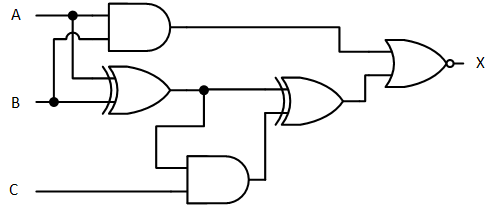
\includegraphics[scale=2]{./img/circuit_logique_B.png}
}
\end{figure}


%\bigskip
\vspace*{1.5cm}

%\clearpage

%%%%%%%%%%%%%%%%%%%%%%%%%%%%%%%%

\begin{table}[!ht]
  \centering
  \begin{minipage}{0.50\textwidth}
    \centering

\subsection{(2 points) Remplissez la table de vérité de la formule précédente : }

%\bigskip

\begin{center}
\begin{tabular}{|C{0.75cm}|C{0.75cm}|C{0.75cm} | C{0.75cm}|}
\hline
\cellcolor{black!15} & \cellcolor{black!15} & \cellcolor{black!15}  &  \cellcolor{black!15} \\
\cellcolor{black!15} & \cellcolor{black!15} & \cellcolor{black!15}  &  \cellcolor{black!15} \\
\hline
 & &   & \cellcolor{black!15} \\
 & &   & \cellcolor{black!15} \\ \hline
 & &   & \cellcolor{black!15} \\
 & &   & \cellcolor{black!15} \\ \hline
 & &   & \cellcolor{black!15} \\
 & &   & \cellcolor{black!15} \\ \hline
 & &   & \cellcolor{black!15} \\
 & &   & \cellcolor{black!15} \\ \hline
 & &   & \cellcolor{black!15} \\
 & &   & \cellcolor{black!15} \\ \hline
 & &   & \cellcolor{black!15} \\
 & &   & \cellcolor{black!15} \\ \hline
 & &   & \cellcolor{black!15} \\
 & &   & \cellcolor{black!15} \\ \hline
 & &   & \cellcolor{black!15} \\
 & &   & \cellcolor{black!15} \\ \hline
\end{tabular}
\end{center}

%%%%%%%%%%%%%%%%%%%%%%%%%%%%%%%%

  \end{minipage}
  \hfillx
  \begin{minipage}{0.50\textwidth}
%    \centering

%%%%%%%%%%%%%%%%%%%%%%%%%%%%%%%%

\subsection{(2 points) Déduisez-en la formule des mintermes, ainsi que la formule des maxtermes : }

\bigskip

Mintermes :

%%\vspace*{3.35cm}
%\vspace*{7.22cm}
\vspace*{3.35cm}

%\begin{equation*}
%    \begin{split}
%X = \; & ( \overline{A} \cdot \overline{B} \cdot \overline{C}) \; + \; ( \overline{A} \cdot \overline{B} \cdot C) \; + \; \\
%    & ( \overline{A} \cdot B \cdot C ) \; + \; ( A \cdot \overline{B} \cdot C )
%    \end{split}
%\end{equation*}

\bigskip

Maxtermes :

\vspace*{3.35cm}
%\vspace*{7.22cm}
%\vspace*{11.44cm}

%\begin{equation*}
%    \begin{split}
%X = \; & ( A + \overline{B} + C ) \; \cdot \; ( \overline{A} + B + C ) \; \cdot \; \\
%    & ( \overline{A} + \overline{B} + C ) \; \cdot \; ( \overline{A} + \overline{B} + \overline{C} )
%    \end{split}
%\end{equation*}

  \end{minipage}
\end{table}


%\bigskip
\vspace*{-0.25cm}

%%%%%%%%%%%%%%%%%%%%%%%%%%%%%%%%

\subsection{(2 points) Remplissez le tableau de Karnaugh, formez les groupes, et déduisez-en la formule réduite : }

%\bigskip

\begin{table}[!ht]
  \centering
  \begin{minipage}{0.08\textwidth}
    \centering

\vfillFirst

\_\_

% A

\vfillLast

  \end{minipage}
  \hfillx
  \begin{minipage}{0.37\textwidth}
    \centering

\begin{center}

\_\_  \_\_

% BC

\medskip

%\begin{tabular}{|C{0.75cm} || C{0.75cm}|C{0.75cm}|C{0.75cm}|C{0.75cm}|}
%\hline
% & 00 & 01 & 11 & 10 \\
%\hline
%\hline
% 0 &  1 & 1 & 1 & 0 \\ \hline
% 1 &  0 & 1 & 0 & 0 \\ \hline
%\end{tabular}

\begin{tabular}{|C{0.75cm} | C{0.75cm}|C{0.75cm}|C{0.75cm}|C{0.75cm}|}
\hline
\cellcolor{black!65}  &  \cellcolor{black!15} & \cellcolor{black!15} & \cellcolor{black!15} & \cellcolor{black!15} \\
\cellcolor{black!65}  &  \cellcolor{black!15} & \cellcolor{black!15} & \cellcolor{black!15} & \cellcolor{black!15} \\
\hline
\cellcolor{black!15}  &  & & & \\
\cellcolor{black!15}  &  & & & \\ \hline
\cellcolor{black!15}  &  & & & \\
\cellcolor{black!15}  &  & & & \\ \hline
\end{tabular}
\end{center}

  \end{minipage}
  \hfillx
  \begin{minipage}{0.55\textwidth}
    \centering

\vfillFirst

\phantom{42}

% $ X = ( \overline{A} \cdot \overline{B} ) \; + \; ( \overline{A} \cdot C ) \; + \; ( \overline{B} \cdot C ) $

\vfillLast

  \end{minipage}
\end{table}

%%%%%%%%%%%%%%%%%%%%%%%%%%%%%%%%%%%%%%%%%%%%%%%%%%%%%%%%%%%%%%%%%%%%%%%%%%%%%

%\vfillFirst
%
%\begin{center}
%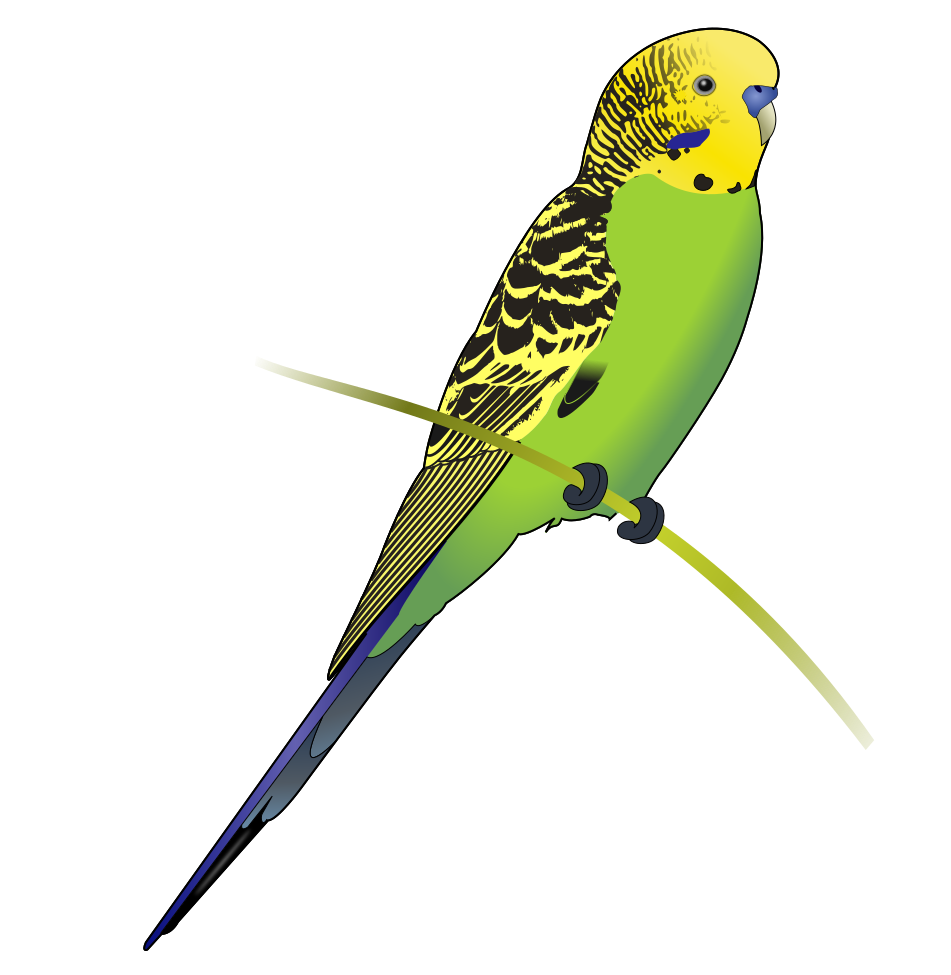
\includegraphics[scale=0.2]{img/others/Budgerigar_diagram.png}
%\end{center}
%
%\vfillLast

\clearpage


%\thispagestyle{empty}

\vfillFirst

\begin{center}

\begin{LARGE}
\textbf{SUJET B}

\bigskip

\textbf{\MakeUppercase{\TitreMatiere}}
\end{LARGE}

\end{center}

\vfillLast

\end{document}
